\chapter{Principe de la solution envisagée}
\label{chap:sol}

  Notre solution est découpée en trois étapes incrémentales. Dans un premier
  temps, nous allons rétablir le procédé de migration de processus
  mono-thread. Dans un second temps, nous ajouterons le support du
  multi-thread. Enfin, nous allons ré-implémenter un composant d'ALMOS appelé
  DQDT, responsable de la politique de migration dans le noyau.

  \begin{paragraph}{Remarque:}
    Dans la section~\ref{sec:mono}, le mot \textit{processus} est utilisé pour
    désigner un processus composé d'un seul thread. Dans la suite de ce
    chapitre, à partir de la section~\ref{sec:multi}, on considère que les
    processus ont plusieurs threads.
  \end{paragraph}


  \section{Support des processus mono-thread}
  \label{sec:mono}

    Cette première étape à pour but de mettre en place deux mécanismes:
    \benumline \item la migration de processus entre noyaux \item la création
    distante de processus\eenumline. Pour compléter ces deux objectifs, il est
    nécessaire de définir l'ensemble des structures partagées par les processus,
    lesquelles devront nécessairement être maintenues cohérentes tout au long de
    l'exécution.

    \subsection{Principes}

      \subsubsection{Rappels}

        L'appel système \texttt{fork()} est la seule et unique manière de créer
        un processus dans un système UNIX. Lorsqu'un processus fait appel à
        cette fonction, un processus identique à l'appelant est créé. L'appelant
        est appelé \textit{père}, et le résultat est appelé \textit{fils}. Le
        fils étant une copie de son père, son exécution commence juste après
        l'appel système \texttt{fork()}.

        Pour qu'un fils exécute un autre programme que celui du père, il faut
        utiliser l'appel système \texttt{exec()}. C'est lui qui permet de
        remplacer le code exécuté par un processus.\\

        Dans la très grande majorité des cas, un appel à \texttt{fork()} est
        suivit d'un appel à \texttt{exec()}. C'est la principale manière de
        lancer des applications différentes dans un système\footnote{Voir
          \texttt{posix\_spawn()} pour une alternative.}. Un exemple
          d'utilisation de ces deux fonctions est donné par le
          Listing~\ref{lst:fork-exec}.

        \lstinputlisting[label={lst:fork-exec}, caption=Utilisation de
          \texttt{fork-exec}. La valeur de retour de \texttt{fork()} permet de
          différencier si le processus en cours d'exécution est le père ou le
          fils.]{include/code/example.c} \FloatBarrier

      \subsubsection{Migration}

        La migration de processus repose sur le mécanisme des RPC du
        noyau. Cette opération consiste à déplacer un processus, pendant son
        exécution, dans un nouveau noyau. Pour déplacer un processus, il faut
        envoyer les informations nécessaires au noyau destinataire pour qu'il
        puisse reconstruire l'espace virtuel du processus. On a notamment besoin
        des adresses de début et de fin:
        \begin{itemize}
          \item de la pile utilisateur
          \item du tas
          \item du code
          \item des arguments
          \item des données
        \end{itemize}
        Pour l'identification et de l'exécution, il faut envoyer les
        informations suivantes:
        \begin{itemize}
          \item le \texttt{pid}
          \item l'identifiant du noyau d'origine
          \item le \texttt{pid} sur le noyau d'origine
          \item l'identificateur de groupe
          \item la priorité
          \item la politique d'ordonnancement\\
        \end{itemize}

        La migration n'est pas explicite pour le programmeur. Elle est à
        l'appréciation de la DQDT, présentée en section~\ref{sec:dqdt}. On veut
        simplement ici mettre en place un mécanisme via RPC permettant de migrer
        un processus à n'importe quel moment de son exécution.

      \subsubsection{Création distante}

        Migrer un processus pendant sa création, donc lors du \texttt{fork()}
        est une erreur. En effet, après avoir déplacé toutes les données du fils
        sur le nouveau noyau, la probabilité que ce dernier fasse un
        \texttt{exec()} est très grande. Par cet appel, il écrasera toutes les
        données que l'on aura déplacées juste avant. On aura donc payé le coût
        de la migration pour rien.\\

        Pour implémenter ce mécanisme, nous avons choisi de nous baser sur
        l'appel système \texttt{exec()}. Nous allons le modifier en ajoutant un
        appel aux fonctions de la DQDT. Si en retour le noyau s'aperćoit que le
        processus doit être migré, alors les informations citées précédemment
        seront envoyées. Ici, les données les plus importantes à transmettre
        sont le code et les arguments qui sont spécifiés dans l'appel
        \texttt{exec()} (voir Listing~\ref{lst:fork-exec}). En effet, on veut
        que le processus qui sera créé exécute un nouveau code et pas celui de
        son père.\\

        Attendre un appel à \texttt{exec()} pour effectuer la migration permet
        de ne pas briser la localité spatiale des processus ayant un lien de
        parenté, et qui par définition accèdent aux mêmes données. On pense par
        exemple au navigateur web Firefox, qui gère ses onglets en utilisant un
        processus complet et non plus un thread~\citep{mozillaElectrolysis}.\\

        On note qu'un processus qui crée beaucoup de fils sans faire d'appel à
        \texttt{exec()} ne représente pas une menace pour la stabilité du
        système. En effet, au bout d'un temps $T$ borné, la DQDT verra la
        surchage engendrée par tous ces processus. Les mécanismes de migration
        expliqués précédemment seront alors activés.

        \begin{paragraph}{Remarque:}
          Un appel à \texttt{exec()} ne migre pas forcément un
          processus. Celle-ci se fait selon la politique de la DQDT.
        \end{paragraph}


    \subsection{Maintien de cohérence}

      Comme nous l'avons vu précédemment, ces deux opérations représentent un
      enjeux quant aux structures de données que contiennent les processus, et
      surtout celle qu'ils partagent. Nous avons identifié les structures
      suivantes comme étant problématiques dans notre cas:
      \begin{itemize}
      \item les descripteurs de fichiers ouverts
      \item les zones mémoires
      \end{itemize}

      Les descripteurs de fichiers contiennent des données qui doivent être
      maintenues cohérentes\footnote{C'est une obligation de la norme
        POSIX~\citep{posix2013}, norme que le noyau ALMOS a choisi de
        respecter.}. Ces informations sont l'offset et le compteur de
      référence\footnote{Uniquement dans le cas du multi-thread}. L'offset
      indique la position à laquelle se trouve le processus dans un fichier. Le
      compteur de référence permet de savoir combien de processus ont ouvert le
      même fichier.

      Lorsqu'un processus ouvre un fichier puis crée un fils, les modifications
      du père doivent être visibles pour le fils, et inversement. Or, chaque
      modification déplace la tête de lecture. Afin de maintenir la cohérence
      dans le fichier, la valeur de l'offset doit être la même pour tous les
      processus ayant ouvert le fichier.

      Dans les sytèmes UNIX, chaque processus à son espace virtuel et ne peut
      pas accéder à celui des autres. Néanmoins, les noyaux permettent d'allouer
      de la mémoire en mode \texttt{SHARED}. Ainsi, deux processus peuvent se
      partager une certaine zone mémoire et ainsi échanger des
      informations. Pour des raisons évidentes, ces zones mémoires partagées
      doivent impérativement être cohérentes entre les processus\footnote{On
        parle ici du contenu de la mémoire, pas de la structure la représentant,
        qui elle est propre aux processus.}.

      %% \begin{paragraph}{Remarque:}
      %%   Tous les processus n'ont pas de zones mémoire partagées avec d'autres
      %%   par défaut. Ainsi, la cohérence de ces dernières n'est pas la priorité
      %%   ici. Nous voulons d'abord être capable de gérer les descripteurs de
      %%   fichiers, qui sont partagés par défaut \texttt{stdin, stdout} et
      %%   \texttt{stderr} sont tous les trois des fichiers et sont ouverts par
      %%   tous les processus en permanence.
      %% \end{paragraph}


    \subsection{Accélération de la migration}

      Afin de faciliter le maintien de la cohérence et surtout accélérer la
      migration, nous allons redéfinir l'implémentation des descripteurs de
      fichiers et des zones mémoires. Il est nécessaire de s'abstraire de
      l'utilisation des pointeurs qui deviennent incorrects lorsqu'un processus
      change de noyau. En effet, une adresse dans un noyau $N$ n'est pas
      toujours significative dans un noyau $N'$. Un bon exemple pour illustrer
      notre cas est celui des processus père/fils. Chaque processus doit savoir
      qui est son père, et possède un pointeur en direction de la \texttt{struct
        task} de ce père. Si le fils est migré sur un nouveau noyau, cette
      adresse est devient obsolète.

      Nous allons donc réduire au maximum le nombre de pointeurs, et notamment
      ceux utilisés pour gérer les descripteurs de fichiers ouverts ainsi que
      les zones de mémoire virtuelle d'un processus. Supprimer ces pointeurs
      implique de devoir changer l'implémentation de la structure de données
      utilisée pour stocker toutes les informations. Nous allons utiliser des
      tableaux pour enregistrer les informations sur les fichiers ouverts par
      les processus. Ces tableaux seront plus faciles à migrer puisqu'ils
      s'agira seulement d'en faire une copie dans la mémoire du noyau
      destinataire.

      Nous avons actuellement deux solutions à l'étude et aucune n'a pour
      l'instant été choisie:
      \begin{itemize}
        \item utiliser une table de hachage par calcul
        \item utiliser une table de hachage chainée
      \end{itemize}

      Quelque soit la solution envisagée, les entrées et sorties sont
      similaires, ce qui nous permet de n'effectuer qu'une seule
      spécification. Nous allons utiliser l'adresse virtuelle accédée comme
      entré de la fonction de hash. En sortie, nous obtenons l'adresse physique
      de la région virtuelle associée.

      \begin{center}
        \texttt{hash(v\_addr) = v\_reg\_addr}
      \end{center}

      La première solution nous garanti de n'avoir qu'une table à
      gérer. Néanmoins, cette gestion est assez difficile dans son
      implémentation. À l'inverse, la table de hash chainée est plus simple à
      mettre en \oe uvre mais les indirections que nous pensont utiliser en
      feront un objet plus complexe que la précédente solution. Ces deux
      possibilités n'ont pour l'instant pas été estimées en terme de coût pour
      le système. Elles restent donc à l'état d'hypothèse jusqu'à ce que l'une
      d'elle s'avère plus efficace.

    %% \subsection{Les descripteurs de fichiers}

    %%   Les \textit{file descriptors} sont une abstraction des systèmes
    %%   d'exploitation permettant aux processus de manipuler des fichiers. Ce sont
    %%   en réalité des structures de données pointant sur une autre structure
    %%   appelée \texttt{struct file}. Celle-ci contient notamment la valeur de la
    %%   tête de lecture, appelé \textit{offset}, et un compteur de référence
    %%   permettant de savoir combien de \textit{file descriptors} pointent sur la
    %%   \texttt{struct file}, \textit{i.e,} combien de fois le fichier à été
    %%   ouvert.

    %%   Lors d'un \texttt{fork()}, un processus enfant héritera de certaines
    %%   informations de son père. La norme POSIX~\citep{posix2013} impose
    %%   notamment qu'un processus enfant doit avoir accès aux fichiers ouverts par
    %%   son père. Néanmoins, un fichier ouvert après un \texttt{fork()} n'est pas
    %%   partagé avec le processus père. Ces deux mécanismes sont illustrés par la
    %%   figure~\ref{fig:file-descriptors}. Le mécanismes des \texttt{inode} est
    %%   introduit juste après.

    %%   \begin{figure}[ht]
    %%     \centering
    %%     \includegraphics[scale=0.5]{file-descriptors-2}
    %%     \caption{Partage d'une \texttt{struct file}. Le processus $A$ appelle
    %%       \texttt{fork()} et crée le processus $C$. Ils partagent la même table
    %%       mais n'ont aucun fichier en commun. $A$ ouvre le fichier
    %%       \texttt{A\_Filename} puis fait un nouveau \texttt{fork()}, créant le
    %%       processus $B$. Ce dernier partage alors la \texttt{struct file}
    %%       pointée par son père.}
    %%     \label{fig:file-descriptors}
    %%   \end{figure}

    %%   Ce partage implique que la tête de lecture soit la même pour les deux
    %%   processus. Lors d'un \texttt{read()} ou d'un \texttt{write()} par le
    %%   processus $A$, celui-ci change la valeur de la tête de lecture. Ce
    %%   changement doit être visible par le processus $B$.

    %%   Cette obligation se révèle problématique dans le cas d'une migration. En
    %%   effet, si un processus enfant est changé de noyau, il est changé d'espace
    %%   d'adressage. Il ne peut donc plus accéder aux données de son père de
    %%   manière directe, et doit utiliser le passage de message. Cette opération
    %%   est très coûteuse, et est source de contention dans le cas des messages de
    %%   cohérence pour la modification de la tête de lecture.\\

    %%   Nous allons changer la gestion des compteurs de références et des
    %%   \textit{offset} du noyau ALMOS. Dans un premier temps, nous allons nous
    %%   abstraire des \textit{file descriptors}. Plutôt que d'avoir des pointeurs
    %%   sur les \texttt{struct file} des fichiers ouverts, nous allons placer au
    %%   sein des processus un tableau contenant ces structures. L'utilisation d'un
    %%   tableau permet de s'affranchir des pointeurs qui sont problématiques lors
    %%   des migrations.

    %%   Ensuite, nous allons changer l'emplacement de l'\textit{offset}. Nous
    %%   allons le déplacer au sein de la \texttt{struct inode}. Un \textit{inode}
    %%   est une structure de donnée représentant le fichier au sein du système de
    %%   fichier. Elle est pointée par les \texttt{struct file} et possède un
    %%   compteur de références fonctionnement sur le même modèle que vu
    %%   précédement.

    %%   \begin{paragraph}{Remarque:}
    %%     La différence entre une \texttt{struct inode} et une \texttt{struct
    %%       file} peut être expliquée comme suit. Soit deux fichiers, dont un est
    %%     un lien symbolique vers l'autre. Ces deux fichiers auront deux
    %%     \texttt{struct file} différentes, car un lien symbolique \textit{est} un
    %%     fichier. Néanmoins, il n'y a qu'un seul fichier \textit{réel} sur le
    %%     disque, qui est matérialisé par sa \texttt{struct inode}. Chaque
    %%     \textit{inode} est unique sur le système.\\
    %%   \end{paragraph}

    %%   Le fait de gérer l'offset d'un fichier directement dans l'\textit{inode}
    %%   nous assure par construction de la cohérence de la valeur de la tête de
    %%   lecture lors de tous les accès, quelque que soit la localisation du
    %%   processus effectuant l'opération. La migration d'un processus sera
    %%   d'autant plus facilitée puisqu'il suffira simplement de copier le tableau
    %%   des \texttt{struct file} du père, l'offset étant gérer dans
    %%   l'\textit{inode}.


    %% \subsection{Les zones mémoire}

  \section{Ajout du multi-thread}
  \label{sec:multi}  

    Une fois le support des processus mono-thread en place, nous allons ajouter
    le support du multi-thread. Cette opération s'avère très délicate, et
    représente probablement l'étape la plus compliquée de ce stage.\\

    Dans la section~\ref{sec:mono}, nous avons présenté les structures de
    données critiques dans le cas d'applications se basant sur des processus et
    non des threads. Nous allons à présent nous intéresser à ces derniers. Après
    étude du problème, nous avons considéré les structures suivantes comme
    problématiques lors que la migration de threads (en plus de celle vues
    en ~\ref{sec:mono}):
    \begin{itemize}
      \item la table des pages
      \item les signaux
    \end{itemize}  

    \subsection{Les processus hybrides}

      Dans la thèse d'\citet{almaless2014universite}, on trouve un des concepts
      clé du noyau ALMOS: les processus hybrides. Partant du principe que la
      notion de thread n'est pas adaptée pour le traitement de la localité des
      accès mémoire,\citeauthor{almaless2014universite} propose de redéfinir la
      notion de processus et de thread. Un processus hybride contient des
      threads qui ont leur propre espace virtuel qui n'est plus accessible par
      les autres threads du processus. Le noyau maintien néanmoins la cohérence
      entre ces espaces. L'intérêt des processus hybride est double:
      \begin{itemize}
        \item on évite le goulot d'étranglement sur la table des pages
          (présentée ci-après)
        \item les espaces virtuels des threads ne sont plus stockés dans le
          processus mais son indépendants, on a donc économiser de la place dans
          la mémoire virtuelle du processus
      \end{itemize}

      Par manque de temps, ce concept n'a pas été implémenté dans le noyau
      ALMOS. Nous allons donc devoir le mettre en place, avec dans un premier
      temps l'objectif d'avoir une table des pages distribuée entre les
      threads.\\

      La table des pages est la structure de données des processus contenant les
      traductions des adresses virtuelles en adresses physiques. Chaque
      processus possède sa propre table des pages. Tous les threads d'un
      processus accèdent de manière atomique à cette table lorsqu'ils veulent
      ajouter une entrée. Ces accès seront problématiques en cas de miss TLB
      fréquents.\\

      Le problème de cette structure est sa granularité de partage: on considère
      un processus entier comme propriétaire. Si l'on migre un thread du
      processus sur un autre noyau, ce dernier accèdera par passage de messages
      à la table, ce qui n'est pas envisageable pour des raisons de
      performances. Il faut donc copier la table des pages entièrement, ce qui
      n'est pas gratuit, et maintenir ensuite une cohérence entre toutes les
      tables répliquées dans les clusters. En prenant en compte le fait que
      chaque processus possède une table de page, les surcoûts liés aux
      communications apparaîssent rapidement.

      Pour répondre à cette problématique, nous allons intégrer une nouvelle
      granularité pour la table des pages en les affectant par thread et non par
      processus. Chaque table contiendra certaines pages communes avec les
      autres threads du processus, mais aura également ses propres pages. Le
      mécanisme proposé est illustré par la figure~\ref{fig:almos-page-table}.

      \begin{figure}[ht]
        \centering
        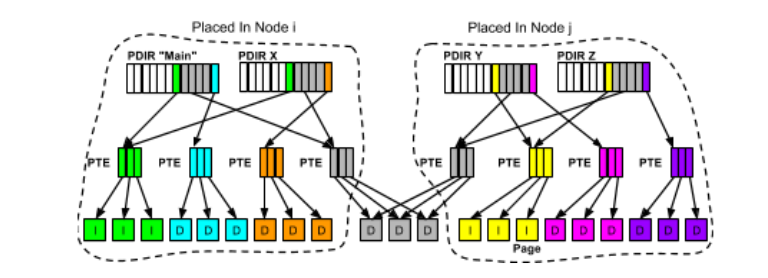
\includegraphics[width=\textwidth]{almos-page-table}
        \caption{Organisation de la table des pages pour quatre threads d'un
          même processus. Deux threads sont placés sur un cluster $I$, et deux
          sur un cluster $J$. Les threads partagent certaines pages de données
          et d'instruction, parfois entre clusters, mais ont également leur
          pages privées~\citep{almaless2014universite}.}
        \label{fig:almos-page-table}
      \end{figure}

      Cette solution permet de minimiser le coût de la cohérence entre tous les
      réplicas des tables et permet également d'alléger les accès atomiques. En
      effet, une application massivement parallèle minimisera les dépendances de
      données entres threads, et donc les pages communes.


    \subsection{Les signaux}

    %% \todo{Vérifier si les signaux sont par threads ou par processus.} C'est par
    %% processus : \texttt{man 7 signal} $\rightarrow$ ``The signal disposition is
    %% a per-process attribute: in a multithreaded application, the disposition of
    %% a particular signal is the same for all threads.''

    %% \todo{Comment retrouver tous les threads d'un processus quand ils ont migré
    %%   sur différents clusters ?} Faut mettre en place un système de \texttt{pid}
    %% ou on peut appliquer des masques. Les MSB du \texttt{pid} contiennent la
    %% valeur du cluster courant, et les LSB la valeur du \texttt{pid} dans ce
    %% cluster. Quand un processus migre, il envoie à son cluster d'origine son
    %% nouveau \texttt{pid} et le cluster d'origine change le \texttt{pid} dans sa
    %% table des processus. On peut savoir que c'est un \texttt{pid} distant
    %% puisque le cluster aura dans son tableau un pid dont les MSB ne
    %% correspondent pas à son \texttt{id}.

      Dans cette partie, nous allons devoir mettre en place des mécanismes pour
      la transmission des signaux lorsque les threads sont distribués sur
      plusieurs noyaux. En effet, la norme POSIX stipule que la portée des
      signaux est un processus dans son ensmble\footnote{Extrait de \texttt{man
          7 signal} : ``The signal disposition is a per-process attribute: in a
        multithreaded application, the disposition of a particular signal is the
        same for all threads.''}.

      Pour cela, il faudra redéfinir la notion de \texttt{pid}. Un \texttt{pid}
      sera découpé en deux parties \benumline \item la partie haute indiquera la
      valeur du cluster sur lequel s'exécute le thread \item la partie basse
      donnera la valeur classique du \texttt{pid} sur ce
      cluster\eenumline. L'application d'un masque sur le champ \texttt{pid}
      permettra alors d'obtenir l'information souhaitée.

      Après une migration, un processus envera son nouveau \texttt{pid} au noyau
      d'origine, qui le modifiera dans sa table des processus. Ainsi, le noyau
      d'origine des processus connait en permanence la localisation de ses fils
      sur la machine. Ce mécanisme nous permet de pouvoir transmettre les
      signaux.


  \section{La DQDT}
  \label{sec:dqdt}

    Cette partie du stage doit être considérée comme ``optionnelle''. La
    réimplémentation de ce composant est un besoin réel pour ALMOS, néanmoins
    cela implique que les étapes présentées précédemment respectent l'échéancier
    que nous verrons au chapitre~\ref{chap:schedule}.\\

    La DQDT, pour \textit{Distributed Quaternary Decision Tree}, est le
    composant d'ALMOS assurant une vision cohérente et temps-réel\footnote{C'est
      un abus de langage qui est fait ici. Nous voulons simplement montrer que
      la DQDT permet d'avoir en permanence les taux d'utilisation des 4096
      processeurs de la plateforme.} de l'utilisation des ressources. Dans la
    version d'\citet{almaless2014universite}, la DQDT repose sur des serveurs
    répliqués dans tous les clusters. Chaque processeur physique représente une
    feuille de la DQDT. Ces serveurs récupèrent les informations sur
    l'occupation des processeurs de la machine, et construisent une moyenne
    d'utilisation pour chaque cluster. Cette information est stockée dans un
    n\oe de l'arbre. Chaque étage de l'arbre représente un niveau
    d'abstraction. Comme le montre la figure~\ref{fig:dqdt-logical}, le premier
    niveau, en noir, est celui des processeurs. Le second niveau, en bleu, est
    celui du cluster, et le dernier, en rouge, regroupe quatre clusters. Ces
    niveaux sont matérialisés par les étages de l'arbre, comme le montre la
    figure~\ref{fig:dqdt-tree}.\\

    \begin{figure}[ht]
      \begin{subfigure}[b]{0.5\textwidth}
        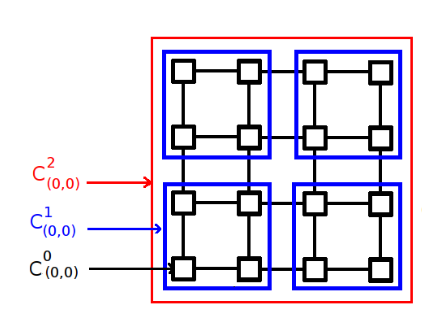
\includegraphics[scale=0.4]{dqdt-logical}
        \caption{Découpage de la plateforme}
        \label{fig:dqdt-logical}
      \end{subfigure}
      \begin{subfigure}[b]{0.4\textwidth}
        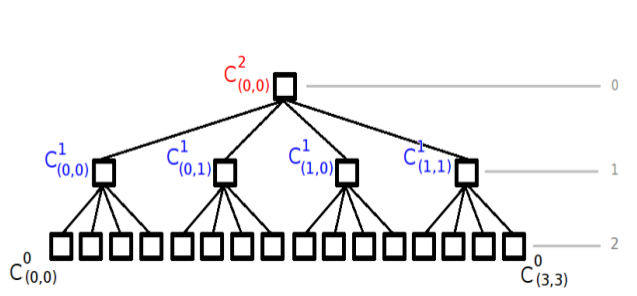
\includegraphics[scale=0.4]{dqdt-tree}
        \caption{Représentation du découpage}
        \label{fig:dqdt-tree}
      \end{subfigure}
      \caption{Construction de la DQDT~\citep{almaless2014universite}.}
    \end{figure}

    La DQDT, comme la plupart des composant noyaux d'ALMOS, repose sur le
    mécanisme de la mémoire virtuelle répartie entre les clusters. Si l'on passe
    ALMOS en mode multi-noyau, les serveurs de la DQDT ne peuvent plus
    communiquer grâce à la mémoire virtuelle. Ils sont obligés d'utiliser le
    passage de messages entre les noyaux.

    Notre but est donc de changer le schéma de communication de la DQDT. Deux
    techniques peuvent être utilisées:
    \begin{itemize}
      \item nous voulons avoir une solution portable sur n'importe quelle
        architecture matérielle : nous allons utiliser le passage de messages
      \item nous voulons avoir une solution efficace sur l'architecture TSAR :
        nous allons profiter des mécanismes matériels nous permettant d'accéder
        directement à la mémoire physique des clusters voisins.
    \end{itemize}

    Nous implémenterons d'abord une version efficace sur TSAR, puis s'il nous
    reste du temps, nous implémenterons une solution générique.
